

\section{Introduction}

A memory allocator is a key component that could significantly impact the performance and memory consumption of the corresponding applications. We performed an experiment on applications of PARSEC~\cite{parsec}, and stress tests of Hoard~\cite{Hoard}, with multiple well-known memory allocators. These allocators include two versions of Linux allocators (glibc-2.28 and glibc-2.21), TcMalloc~\cite{tcmalloc}, \texttt{jemalloc}~\cite{jemalloc}, and Hoard~\cite{Hoard}. Figure~\ref{fig:motivation} shows partial performance results, where all data in the figure is normalized to that of the Linux default allocator (glibc-2.28). We have the following observations: (1)~the performance difference with different allocators can be as large as $47\times$, i.e. \texttt{cache-thrash} with TcMalloc; (2)~No allocator performs consistently the best across all tested applications, indicating the importance of identifying the internal reason.
%, indicating that sometimes spending additional effort toward optimizing the application code may have a smaller  impact than simply switching to a better-suited allocator. (2)~No allocator performs consistently the best across all tested applications, indicating the importance of identifying the internal reason. 

\begin{figure}[!ht]
\centering
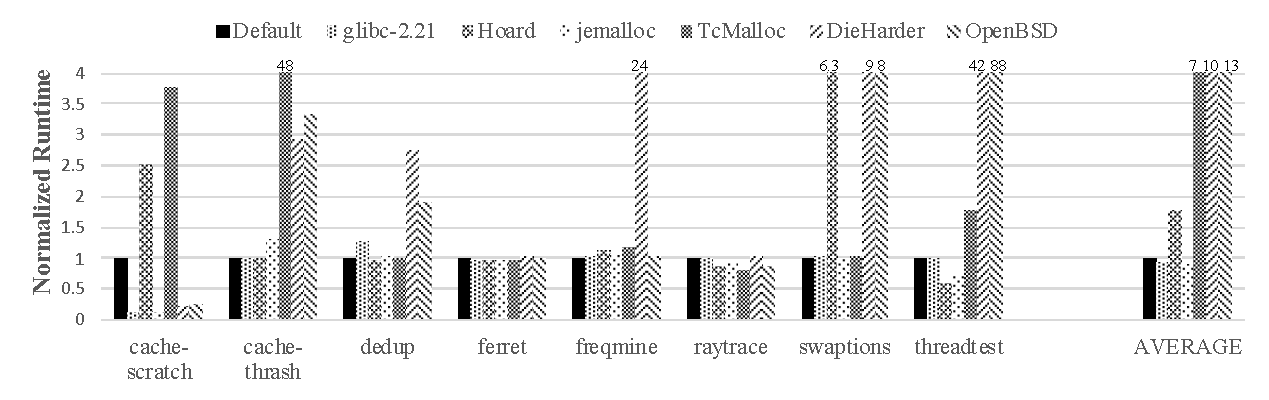
\includegraphics[width=0.9\columnwidth]{figures/regular-performance}
\caption{Performance Impact of Allocators\label{fig:motivation}}
\end{figure}

\begin{figure}[!ht]
\centering
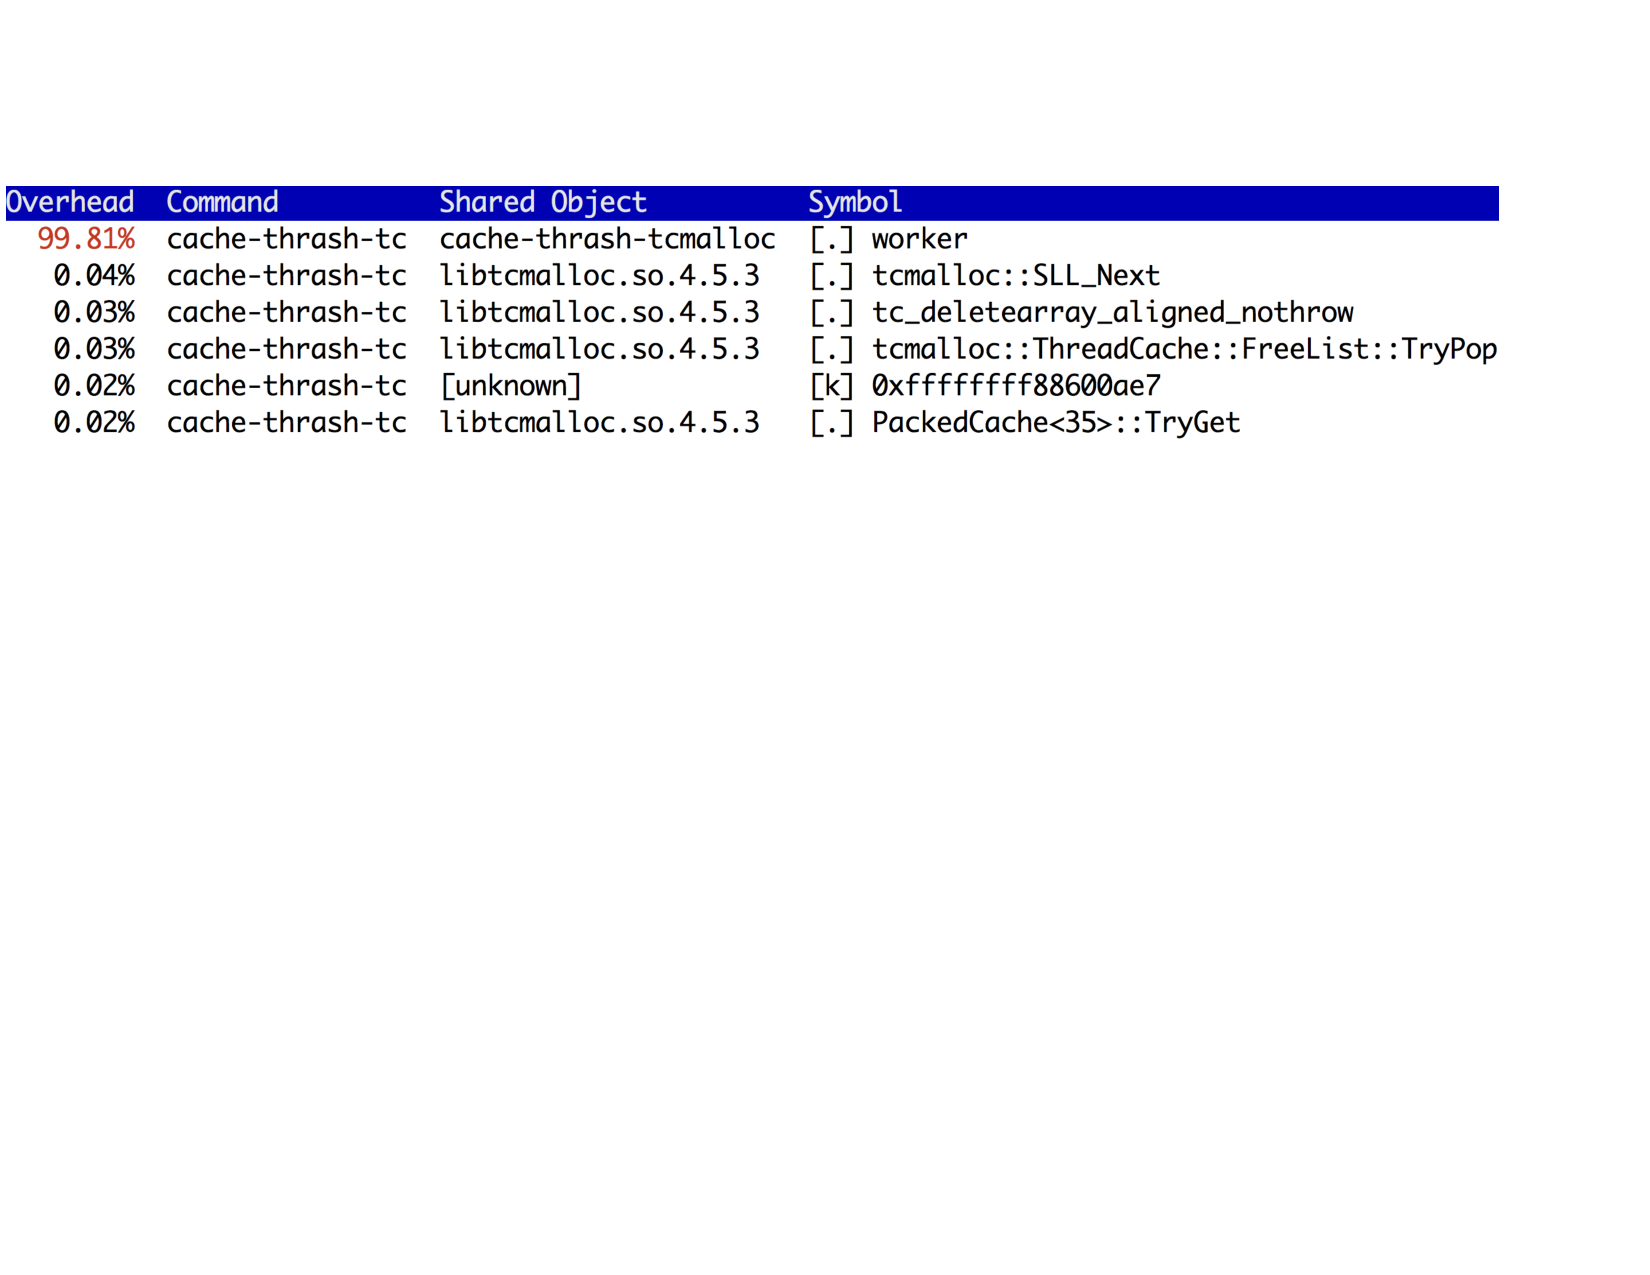
\includegraphics[width=0.9\columnwidth]{figures/perf-cache-thrash-tcmalloc}
\caption{Profiling results of \texttt{perf}. \label{fig:mot1}}
\end{figure}

However, none of existing profilers can identify the inherent reason of the performance slowdown caused by an allocator. General profilers, such as \texttt{gprof}~\cite{DBLP:conf/sigplan/GrahamKM82} and \texttt{perf}~\cite{perf}, only report the time accumulation of different functions, and \texttt{Coz}~\cite{Coz} presents a quantitative performance impact of improving a particular region of code. We used \texttt{perf}, \texttt{gprof}, and \texttt{Coz} to analyze the performance issue of TcMalloc on \texttt{cache-thrash}, since it runs around $48\times$ slower than the default Linux allocator. As shown in Figure~\ref{fig:mot1}, \texttt{perf} reports the \texttt{worker} function as the primary function to focus on, which unfortunately has nothing to do with the slowdown reason. \texttt{gprof} reports the similar results as \texttt{perf}. Instead, \texttt{Coz} reports reports the program lines of exercising these objects with passive false sharing issues, i.e. lines 85-87 of \texttt{cache-thrash.cpp}, and predicts that the performance can be improved up to \textbf{10\%} if these lines can be improved by 100\%. However, \texttt{Coz} does not pinpoint that the performance slowdown is actually caused by the allocator, as discussed in Section~\ref{sec:effectiveness}, and its prediction on the performance impact is obviously much smaller than the real one ($48\times$).

%However, they cannot identify the performance issues of a memory allocator, due to the following reasons. \texttt{First}, they do not collect allocator-specific data, and provide no metrics for evaluating an allocator. For instance, \texttt{perf} may report the number of cache misses, but it is impossible to know how many of these events are actually caused by the allocator. Without that information, it is unable to determine whether a performance issue is originating from the allocator. \texttt{Second}, none of these tools collect kernel contention information, an important issue related to the allocator. For instance, the glibc-2.21 allocator slows down the performance of \texttt{dedup} by more than 20\%, which is caused by frequent \texttt{madivse} system calls that directly lead to the heavy kernel contention. However, such an important issue cannot be identified by general profilers~\cite{DBLP:conf/sigplan/GrahamKM82, Coz, perf}%, \todo{as discussed in Section~\ref{}}.
%Third, none of these profilers report the application friendliness of an allocator, which is critical to understanding the performance slowdown caused by a particular allocator.   

Existing allocation profilers, such as \texttt{mprof}~\cite{Zorn:1988:MAP:894814}, Mtrace~\cite{mtrace}, Mtrace++~\cite{Lee:2000:DMM:786772.787150}, \texttt{TcMalloc} profiler~\cite{tcmalloc-profiler}, or CLR profiler~\cite{lupasc2014dynamic}, mainly focus on how an application uses the memory. For instance, \texttt{mprof} attributes memory allocations to different allocation sites, and reports memory leaks and a direct allocation table that shows the memory usage of functions~\cite{Zorn:1988:MAP:894814}. The \texttt{TcMalloc} profiler reports heap usage of different allocation sites, and locates memory leaks~\cite{tcmalloc-profiler}. That is, these allocation profilers cannot tell the design issues of a particular allocator. 

Due to the obvious importance of a memory allocator, it is emergent to design a profiler that could pinpoint design/implementation issues of an allocator. This profiler should be able to profile different allocators so that there is no need to reinvent the wheel for allocator designers, when they design a new allocator or improve an existing allocator. More importantly, the profiler should also benefit normal users, not just limit to allocator designers. This paper presents such a profiler--\MP{}--that focuses on different aspects of an allocator that will benefit both allocator designers and normal users. 

\MP{} will benefit normal users in the following ways. First, \MP{} can predict the performance slowdown caused by the current allocator, which clearly indicates whether it is necessary to improve the allocator or switch to a new allocator. Second, \MP{} will report the detailed memory waste caused by the allocator. Therefore, users may utilize a different allocator if memory waste is a big concern for users, since a high-performant allocator may actually waste more memory. Third, \MP{} will also report multiple metrics of application-friendliness, which tells whether an allocator is tapped with allocation/deallocation pattern or access pattern of a particular application. As described above, a performant allocator like TcMalloc may be  not suitable for a particular application (e.g., \texttt{cache-thrash}). 
% which helps determine whether the current allocator is suitable for this application or not.
 
\textit{The novelty (and challenge) of \MP{} lies in its decision of what to profile and how to profile to satisfy the precision and efficiency}. First, \MP{} profiles the performance impact of memory allocations/deallocations, which will directly affect the performance of running an application. It is straightforward to utilize the time (cycles) of each allocation and deallocation as the metrics, which can be collected by simply intercepting memory allocations and deallocations. However, this method still has multiple issues. First, the data can be misleading or without pointing out the real design issue, since allocators typically handles small and big objects differently. Therefore, \MP{} differentiates the data based on its category, small or big objects. Second, multiple reasons may cause a slow  management operation, such as too many instructions, cache misses or page faults (hardware-related), user-space and kernel-space contention. Therefore, \MP{} further utilizes hardware performance monitor units (PMUs) to collect hardware related events (instructions, cache misses, or page faults), and intercepts synchronizations and memory-related system calls to obtain user-space and kernel contention. The data will be also collected based on the category of allocations, helping understand the particular design issue inside. For instance, glibc-2.21 invokes a large number of \texttt{madvise} systems calls for the \texttt{dedup} application~\cite{madvise}, which actually causes over 20\% slowdown. \MP{} is able to report such issues by intercepting memory-related system calls. 

Second, \MP{} aims to report different types of memory wastes introduced by an allocator. It is easy to measure internal fragmentation, which could be collected by summing up the difference between a requested size with its corresponding class size. However, it is challenging to measure other wastes, such as memory blowup and external fragmentation. Memory blowup occurs when memory deallocations from one thread cannot be utilized to satisfy subsequent memory requests from other threads~\cite{Hoard}, due to the utilization of per-thread heaps. However, this definition cannot be utilized directly to collect the total memory blowup, and it also does not specify how to update upon the consequent deallocation and re-allocation. \MP{} computes memory blowup based on the following observation: \textit{all freed objects of a size class represent the upper bound of memory blowup for this size class}. \MP{} further proposes a practical solution to compute the memory blowup, and then computes the external fragmentation afterwards. 

Third, \MP{} will identify application-friendliness of an allocator. \MP{} proposes to profile the following metrics, including cache utilization rate, page utilization rate, passive/active false sharing, and cache invalidation rate (outside allocations/deallocations). Further, \MP{} proposes to employ PMUs to sample memory accesses in order to collect these parameters practically. To collect cache utilization rate, \MP{} tracks used bytes for every cache line, and then updates the overall cache utilization rate upon every access. Overall, these parameters will help users to understand the performance degrade on a specific application. As an example, \MP{} reports that the passive false sharing is the direct reason for TcMalloc's low performance on \texttt{Cache-trash} application.




%\textit{First, it provides multiple metrics that help allocator developers to discover design issues of a particular memory allocator}. \textit{Second, it helps normal programmers to determine whether an application's performance or scalability issue is caused by a memory allocator}. 
%\MP{} reports multiple metrics for users to judge whether the allocator is the culprit of the performance/scalability issue or not. 
%If so, programmers can fix the issues affecting the allocator or switch to a better-suited allocator altogether, instead of focusing on the application itself. 
%\textit{Third, mmprof reports different types of memory overhead caused by an allocator, helping normal users analyze memory overhead issues.} 
%If the memory overhead is mainly caused by an allocator, e.g., TcMalloc uses $1.8\times$ more memory than the default Linux allocator for \texttt{swaptions}, then it is less useful to reduce the memory usage of this application. Instead, a more memory-efficient allocator should be employed.   

% What is the design principle? 


% What to do? and How to do?
%\MP{} aims to evaluate all important aspects of memory allocators, such as performance, memory, scalability, and application-friendliness. \MP{} is based on the observation that memory allocators share many commonalities, making it feasible to design a general profiler for different allocators. First, they interact with other components of the system similarly: they provide the same API's to applications (e.g., \texttt{malloc()} and \texttt{free()}), invoke a limited set of system calls (e.g., \texttt{mmap} and \texttt{sbrk}), and employ a set of thread synchronization primitives for synchronization. Second, memory allocators share similar memory management policies, such as belonging to either sequential or BiBOP-style memory layout types, employing per-thread heaps, differentiating small and large objects, and managing small objects with different size classes (where more details are discussed in Section~\ref{sec:allocator}). Therefore, \textit{mmprof employs several common mechanisms to perform the profiling, while utilizing a configuration file to understand the differences between various allocators}.    

%\MP{} intercepts the interactions between an allocator and other components such as the application, the \texttt{pthreads} library, and the underlying operating system, in order to collect the detailed data for each allocation/deallocation request, and the contention information for both user and kernel space.  \MP{} employs simple counters and timestamps for collecting basic data, such as the number of invocations. In addition, \MP{} further employs the CPUs' Performance Monitoring Units (PMU's) to collect hardware-based events, and attributes them each to allocations/deallocations. The PMU's avoid the requirement of explicitly modify source code, and provide more insights about a particular design issue. \MP{} also proposes practical solutions to evaluate certain important metrics, such as cache/page utilization rates, memory blowup, active/passive false-sharing, and kernel contention. Although some of these metrics have been proposed before~\cite{Hoard}, \textit{mmprof is the first to evaluate them quantitatively}. In order to enable the comparison between different executions, \MP{} normalizes the data to each allocation, each access, and each unit of time.  

% How we are going to implement this? 
%\MP{} uses the hardware Performance Monitor Units (PMU) and RDTSC timestamps widely available in modern CPUs to perform the profiling. \MP{} achieves three goals to act as a practical memory allocator profiler for real-world programs. First, it should directly work on the executables. Second, it should reveal the overhead and scalability of the allocators themselves. Since the invocations to the memory management functions are synchronous, the efficiency of the allocator has a direct impact on performance. Third, it should quantify the ``application friendliness'' of the memory allocator, a metric to show how well the allocator manages memory for the application, which is drawn from statistics of accesses to different levels of the memory hierarchy.

%(1) When the profiler works directly on the executable, it is difficult to distinguish the behaviors caused by the allocators and those caused by the program code. 
%We face multiple challenges to achieve the goals. (1) The profiler, despite sampling a large number of events and obtaining extensive information, should maintain a low runtime overhead, and should not seriously distort the execution of the profiled targets (e.g. allocator).  (2) The profiler should not only identify the regular design issues (e.g., poor cache locality or poor object reuses) of the allocator, but also reveal the serious issue of interacting with the OS since a poor design may invoke excessive OS system calls and introduce unnecessary kernel contention. (3) A memory allocator may significantly affect the performance of applications, not just limiting to itself, which has never been evaluated quantitively before. (4) The profiler should be able to adapt to different allocators, which is the major target of designing a general profiler.   
%  to be quantified. 
% manage memory outside of its library calls, which is hard to capture and quantify. 
%carefully manage its internal memory allocations to

%To address these challenges, we design \MP{} in a principled way to determine what events to sample and what profile knowledge the sampled events contribute to. Briefly speaking, \MP{} always intercepts the allocator library calls to figure out when the program execution is inside the allocator, during which it samples both performance related PMU events (e.g., cache misses) to determine the implementation issues and intercepts OS kernel calls to understand OS-level contention. When the program execution is outside of the allocator, \MP{} samples specific PMU events to determine cache line- and page-level utilization ratio, and cache contention rate, which could directly and significantly impact the performance of the corresponding applications. To maintain low overhead, \MP{} employs a fast lookup mechanism that enables fast checking on the size information of each object, and on the cache line usage and page usage upon each sampled access. ??(WB) one more sentence about the low overhead?? ??(WB) It allocates its internal memory on ...??

Overall, \MP{} profiles important aspects of memory allocators for the first time, such as performance, memory, scalability, and application-friendliness. Based on our extensive evaluation, \MP{} successfully identifies multiple known and new design issues inside popular allocators, as further described in Section~\ref{sec:effectiveness}. Due to its careful design, \todo{\MP{}'s performance overhead is around $50\%$ and its memory overhead is around $56\%$}. This efficient design reduces \MP{}'s interference to the original execution. \MP{} does not need to the change of the allocator, the application, and the underlying OS, which will be convenient for the employment. 

%\todo{one way to highlight the contribution is to emphasize on the **complex** considerations of designing good allocators and the challenges to identify design problems. We want to let the reviewer know that it's difficult to do. }

\subsection*{Contribution}

Overall, this paper makes the following contributions. 

\begin{itemize}
\item It proposes the first general profiler--\MP{}--to profile different memory allocators, without the need of the change of the allocator and the underlying OS, if an allocator utilizes the standard synchronization.  

\item \MP{} profiles multiple aspects of an allocator that will significantly impact the performance and memory overhead of an allocator, with the assistance of PMUs, time-stamp counters, and simple counters together. 

\item \MP{} proposes multiple practical methods to profile some of these metrics precisely and efficiently for the first time, such as memory blowup, cache/page utilization rate. 
%profile cache/page utilization rate, memory blowup, active/passive false sharing, and kernel contention for the first time.
%, and attributes the data to each allocation and deallocation, helps discover designing issues that cannot be discovered with general profilers.  
 
\item This paper performs extensive experimentation to confirm its effectiveness, performance, and memory overhead.    

\end{itemize} 

\begin{comment}

%\todo{What is new in this tool? Whether it could provide some information that is not available in an existing allocator.}

\begin{itemize}
\item It will quantify application-friendliness, which is not available in existing work, and which helps users to decide which allocator should be used for a specific application. 
\item It will provide the memory usage (overhead) information, such as internal fragmentation, and objects that are not freed but yet which remain unused. 
\item It will provide some information that only exists across multiple profilers, for instance, the average number of instructions of each allocation and deallocation, the average time spent within each allocation and deallocation (PMU sampling will be placed outside of the time span, thus not avoiding an erroneous measurement of how long this allocation and deallocation request has been sampled), whether there are some contentions during allocation (user space and kernel space), how many lock acquisitions.  
\end{itemize}
 	
\end{comment}

\subsection*{Outline}

The remained of this paper is organized as follows. It starts with a motivation example in Section~\ref{sec:motivation}. Section~\ref{sec:background} discusses the background of memory allocators, and the basic idea and challenges of \MP{}. Then Section~\ref{sec:implementation} presents the detailed implementation. After that, Section~\ref{sec:evaluation} shows the results of experiments on different allocators using \MP{}, and Section~\ref{sec:limitation} discusses some limitations. In the end, Section~\ref{sec:relatedwork} discusses related work in this field, and Section~\ref{sec:conclusion} concludes this paper.